\documentclass[10pt,a4paper]{article}
\usepackage[utf8]{inputenc}
\usepackage{amsmath}
\usepackage{amsfonts}
\usepackage{amssymb}
\usepackage{graphicx}
\usepackage{gensymb}
\usepackage{color}
\author{Sebastian Bitzer}
\title{Bayesian decision models based on comparing estimated perceptual variables to a criterion}
\begin{document}

\maketitle

\section{Perceptual decision tasks based on estimation}
We here consider perceptual decision tasks in which a decision maker (agent, or participant in an experiment) has to estimate a continuous perceptual quantity from observations and then has to make a judgement about the estimated quantity in relation to a criterion. The example we predominantly consider here is that the decision maker observes noisy motion in a particular direction observed from a random dot kinematogram and has to state whether the observed motion direction is rotated clockwise or anti-clockwise with respect to a criterion direction. So the decision maker has to estimate the motion direction and compare this to the criterion to make a decision.

\begin{figure}[ht]
\centering
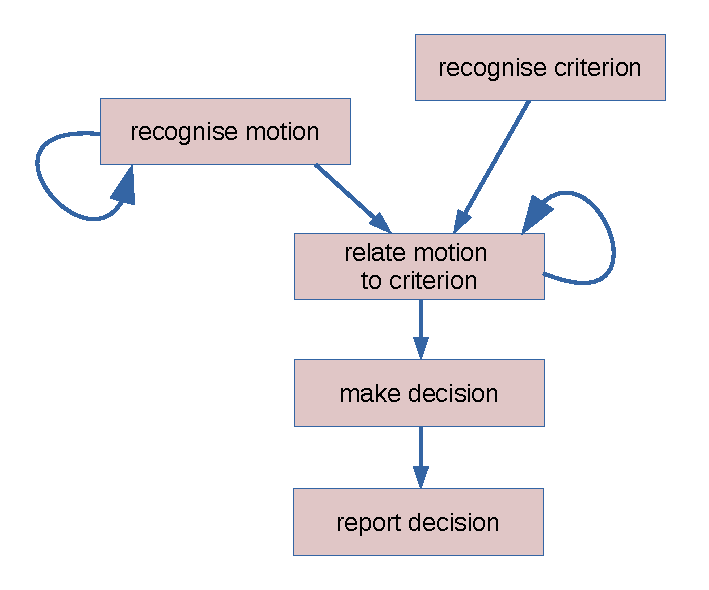
\includegraphics[width=0.7\textwidth]{model_diagram}
\caption{Possible processes involved in making decisions based on estimating a perceptual variable and comparing it to a criterion. Loopy arrows indicate processes in which potentially most time is spent.}
\end{figure}

\section{Model}
\subsection{Most time spent in estimation or comparison?}
We consider two places in which the brain may spent time: during the estimation of the observed motion direction and during the comparison of motion direction to criterion. Although we have previously established that for certain motion directions it may be harder to correctly compare the motion direction to the criterion and, therefore, the comparison process may add variability across trials, I from now on assume that we can ignore this variability. My justification is that I assume that over sufficiently many trials participants have learnt to do the comparison equally well across all motion directions so that the comparison process only adds constant time to the response time across trials. To establish this experimentally we would have to check whether RTs in trials, in which the motion direction switched by more than 90\degree in comparison to the previous trial, are longer than the RTs in trials, in which the motion direction differed by less than 90\degree from that of the previous trial.

So I proceed ignoring contributions from the comparison process for now.


\subsection{Perception as Bayesian estimation}
We assume that the decision maker uses Bayesian inference to estimate the value of a quantity of interest from observations. These observations arrive sequentially and are drawn from this distribution:
\begin{equation}
Y_t \sim p(Y_t | F_t(X))
\end{equation}
where $Y_t$ is the observation at time $t$ and $F_t(X)$ is a feature value that could potentially change over time (when a feature of a stimulus changes in a controlled way during the experiment). $X$ is the underlying quantity that the decision maker tries to infer and $F_t(X)$ expresses that the feature values are a function of this quantity. In the simplest case, $F_t(X) = X$.

The decision maker, not knowing about potential experimental manipulation, has a slightly simpler hypothesis over how observations are generated from the quantity of interest:
\begin{equation}
Y_t \sim \hat{p}(Y_t | X)
\end{equation}
The decision maker then tries to estimate the underlying $X$ from a sequence of observations $Y_1, \dots, Y_T$ by using Bayes formula:
\begin{equation}
\hat{p}(X | Y_1, \dots, Y_T) = \frac{\hat{p}(X)\prod_{t=1}^T \hat{p}(Y_t | X)}{\hat{p}(Y_1, \dots, Y_T)}  
\end{equation}
Equivalently, we can express this in a sequential form using Bayesian belief updating:
\begin{equation}\label{eq:beliefupdate}
\hat{p}(X | Y_{:t}) \propto \hat{p}(Y_t | X) \hat{p}(X | Y_{:t-1})
\end{equation}
where we have used $Y_{:t} = Y_1, \dots, Y_t$ and $\hat{p}(X|Y_{:0}) = \hat{p}(X)$ is the decision maker's prior belief about $X$. Decisions are then made based on the posterior beliefs $\hat{p}(X | Y_{:t})$.

So far we have not made any specific assumptions about what $X$ is and which distributions over $X$ we consider. One possibility is that $X$ is a discrete variable taking on $m$ distinct values: $X \in \{x_1, \dots, x_m\}$, but $X$ can also be continuous.

\subsection{Decisions based on comparison to a criterion}
Perceptual decision making models usually describe the evolution of one or more decision variables where higher values of the decision variable indicate more evidence for one decision alternative compared to another. We can get the desired decision variables as function of the posterior beliefs of the decision maker. Here we handle the case in which the decisions are made as a comparison to a criterion. So our decision variable reflects this criterion which we call $C$ and can be compared to the quantity of interest $X$.

In the simplest case we just want to know whether the estimated quantity $X$ is larger or smaller than the criterion $C$. Then the decision variable could be:
\begin{equation}
DV_< = \hat{P}(X < C | Y_{:t})
\end{equation}
or 
\begin{equation}
DV_> = \hat{P}(X > C | Y_{:t})
\end{equation}
and we would make a decision as soon as either of them exceeds a probability threshold $\lambda$, i.e., when
\begin{equation}
DV_< > \lambda \quad \mathrm{or} \quad DV_> > \lambda.
\end{equation}
But we can also define decision variables based on arbitrary partitions of the different values $X$ can take on. If, for example, we partition $X$ into three different, distinct spaces $\mathcal{A}, \mathcal{B}$ and $\mathcal{C}$ we could define
\begin{align}
DV_\mathcal{A} &= \hat{P}(X \in \mathcal{A} | Y_{:t})\\
DV_\mathcal{B} &= \hat{P}(X \in \mathcal{B} | Y_{:t})\\
DV_\mathcal{C} &= \hat{P}(X \in \mathcal{C} | Y_{:t})
\end{align}
and make a multi-alternative decision as soon as any of these decision variables exceeds $\lambda$.

Staying in two-alternative decisions, a more common decision variable is one which directly compares the probabilities of the two alternatives. For example:
\begin{equation}
DV_{<>} = \frac{\hat{P}(X < C | Y_{:t})}{\hat{P}(X > C | Y_{:t})}
\end{equation}
which is usually expressed in log-space:
\begin{equation}
DV_{l<>} = \log\hat{P}(X < C | Y_{:t}) - \log\hat{P}(X > C | Y_{:t})
\end{equation}
so that evidence for the one alternative (here: $X < C$) is positive while evidence for the other (here: $X > C$) is negative.

\subsection{Difference to DDM}
The DDM can also be formulated in the above Bayesian decision framework. Specifically, to implement the DDM $X \in \{a, b\}$ is binary directly representing decision alternatives $a$ and $b$. In this case, a decision variable $V$ can be defined as
\begin{equation}
V = \log\hat{P}(X=a | Y_{:t}) - \log\hat{P}(X=b | Y_{:t}).
\end{equation}
Applying recursive Bayesian belief updating (Eq. \ref{eq:beliefupdate}) we can obtain a dynamics for $V$:
\begin{align}
V_t &= \log\left[\hat{p}(Y_t | X=a) \hat{P}(X=a | Y_{:t-1})\right] - \log\left[\hat{p}(Y_t | X=b) \hat{P}(X=b | Y_{:t-1})\right]\\
& \begin{aligned}=\log\hat{P}(X=a | Y_{:t-1}) - \log\hat{P}(X=b | Y_{:t-1})\\ + \log\hat{p}(Y_t | X=a) - \log\hat{p}(Y_t | X=b)\end{aligned}\\
&= V_{t-1} + \log\hat{p}(Y_t | X=a) - \log\hat{p}(Y_t | X=b)
\end{align}
so we see that $V$ accumulates the momentary evidence provided by $M_t = \log\hat{p}(Y_t | X=a) - \log\hat{p}(Y_t | X=b)$. To explicitly account for continuous time we can just add the appropriate time step $\Delta t$:
\begin{equation}
V_t = V_{t-1} + \Delta t M_t.
\end{equation}
The usual DDM equation can then be derived by assuming that the sampling distribution $p(Y_t | F_t(X))$ and the likelihood $\hat{p}(Y_t | X)$ are Gaussian with some extra constraints [Bitzer2014].

The point here is that the DDM is a linear accumulator of momentary evidence. That is not the case for $DV_{l<>}$, i.e., there is no linear recursive formula
\begin{equation*}
DV_t = DV_{t-1} + M_t
\end{equation*}
for this decision variable in which $M_t$ is independent of $DV_{t-1}$. This is, because $DV_{<>}$ relates two sums or integrals over the posterior distribution $\hat{p}(X | Y_{:t})$ to each other. This prevents us from separating the momentary evidence provided through the likelihood $\hat{p}(Y_t | X)$ from the previous value of the decision variable. Specifically, the change in the decision variable is:
\begin{equation}
\begin{aligned}
DV_t - DV_{t-1} = &\log \int_{x \in \mathcal{A}} \hat{p}(Y_t | X=x) \hat{p}_\mathcal{A}(X=x | Y_{:t-1})dx\\ &- \log \int_{x \in \mathcal{B}} \hat{p}(Y_t | X=x) \hat{p}_\mathcal{B}(X=x | Y_{:t-1})dx
\end{aligned}
\end{equation}
where we have here assumed continuous $X$ and
\begin{equation}
\hat{p}_\mathcal{A}(X=x | Y_{:t-1}) = \frac{\hat{p}(X=x | Y_{:t-1})}{\int_{x \in \mathcal{A}} \hat{p}(X=x | Y_{:t-1}) dx}
\end{equation}
is the posterior density at the previous time point, but renormalised only within the space of $X$ belonging to alternative $\mathcal{A}$. This means that the evidences for the two alternatives at a given time point compute as the expectation over likelihood values within the space of $X$ defined by the corresponding alternative. The momentary evidence, as their difference, therefore, also depends on the previous accumulated evidence and we cannot formulate a simple linear dynamics for the decision variable.

We can already see now that this will lead to a peculiar dynamics of the decision variable, when the space of $X$ belonging to one of the alternatives is large and in each trial the stimulus only selects a subset of this space. In this situation, starting with a uniform prior over $X$ values, we will initially average likelihood values across the whole space of the alternative. As a result, the change in decision variable will be small, because the expected likelihood values will be small. Later on, however, as the posterior $\hat{p}(X | Y_{:t})$ concentrates around the true, stimulus-provided value of $X$, the evidence for one alternative will be larger, because we will be only averaging relatively large likelihood values. Consequently, we should expect that the decision variable will initially move slowly with small noise, but then picks up speed and is more influenced by noise in the observations.


\subsection{A model for clockwise vs. anti-clockwise rotated motion directions}
In our task we assume that the decision maker first estimates the direction of a noisy motion signal and then compares that to a criterion direction to determine whether the motion is clockwise or anti-clockwise rotated with respect to the criterion. 

\subsubsection{Estimation model}
Directions can be represented by continuous angles and have a special periodic geometry. It is, therefore, not possible to model directions with Gaussian distributions. Common distributions over angles are the von Mises distribution and the wrapped normal distribution, but the latter has no analytic density function. In our model, we thus use the von Mises distribution for the likelihood:
\begin{equation}
Y_t \sim \hat{p}(Y_t | X) = \mathcal{M}(Y_t | X, \hat{\kappa})
\end{equation}
with
\begin{equation}
\mathcal{M}(Y_t | X, \kappa) = \frac{e^{\kappa \cos(Y_t - X)}}{2\pi I_0(\kappa)}
\end{equation}
and also as sampling distribution:
\begin{equation}
Y_t \sim p(Y_t | F_t(X)) = \mathcal{M}(Y_t | F_t(X), \kappa).
\end{equation}
Note that we here use two different precisions: $\kappa$ in the sampling distribution and $\hat{\kappa}$ in the likelihood. These are free parameters of the model. We also express them in terms of $\sigma$ and $\hat{\sigma}$ describing the spread of the distributions instead of the precisions:
\begin{equation}
\kappa = \frac{1}{\sigma^2} \quad \hat{\kappa} = \frac{1}{\hat{\sigma}^2}.
\end{equation}

Ideally we would also find a continuous posterior distribution over $X$, but this is complicated. We might consider it later, but help us for now with a simple discretisation of $X$. This can be motivated from the nature of the experiment in which the stimuli only displayed a small set of motion directions. So we define
\begin{equation}
X \in \{x_1, \dots, x_n\} = \mathcal{X}
\end{equation}
where $n$ is the number of motion directions used in the experiment. The posterior over $X$ then simply becomes
\begin{equation}\label{eq:caposterior}
\hat{p}(X=x_i | Y_{:T}) = \frac{\hat{p}(X=x_i)\prod_{t=1}^T \hat{p}(Y_t | X=x_i)}{\sum_{j=1}^n \hat{p}(X=x_j)\prod_{t=1}^T \hat{p}(Y_t | X=x_j)}
\end{equation}

\subsubsection{Decision/comparison model}
Within a trial the criterion direction $CD$ is fixed and we need to partition the values of $X$, i.e., the possible motion directions, into those corresponding to clockwise rotation denoted as $\mathcal{C}$ and those corresponding to anti-clockwise rotation $\mathcal{A}$. We have to take care when doing this, but we here assume that it has been done. Note, however, that there might be motion directions that neither fall into $\mathcal{C}$, nor $\mathcal{A}$, for example, when $CD = x_i$ for one $x_i$.

We can now define the corresponding decision variable as
\begin{equation}
DV_t^{\mathcal{CA}} = \log \sum_{x \in \mathcal{C}} \hat{p}(X=x | Y_{:t}) - \log \sum_{x \in \mathcal{A}} \hat{p}(X=x | Y_{:t}).
\end{equation}
and make a decision as soon as 
\begin{equation}\label{eq:cacrit}
\left|DV_t^{\mathcal{CA}}\right| > \beta
\end{equation}
where $\beta$ is our decision bound. We can also reformulate $\beta$ as a probability bound which may make it a bit easier to interpret. This works only, when we renormalise such that
\begin{equation}
\sum_{x \in \mathcal{C}} \hat{p}(X=x | Y_{:t}) + \sum_{x \in \mathcal{A}} \hat{p}(X=x | Y_{:t}) = 1.
\end{equation}
Then, the decision criterion defined in Eq. \eqref{eq:cacrit} is equivalent to deciding as soon as
\begin{equation}
\hat{p}(X \in \mathcal{C} | Y_{:t}) > \lambda \quad \mathrm{or} \quad \hat{p}(X \in \mathcal{A} | Y_{:t}) > \lambda
\end{equation}
with
\begin{equation}
\beta = \log\frac{\lambda}{1-\lambda}
\end{equation}
[see Bitzer2014] such that $\lambda$ is the desired posterior probability of an alternative under the assumption that both alternatives together exhaust all possible motion directions. $\lambda$ must be within $(0.5, 1)$.

\subsubsection{Relation to real time}
Although we cannot define a simple, linear dynamics of the decision variable $DV_t^{\mathcal{CA}}$, the definition of the posterior (Eq. \ref{eq:caposterior}) suggests a simple dynamics for the posterior. Because the $DV_t^{\mathcal{CA}}$ is defined as a comparison of two parts of the posterior, the normalisation constant of the posterior cancels and we can here ignore it. The log-posterior is then just
\begin{equation}
\log\hat{p}(X=x_i | Y_{:T}) \propto LP_T^i= \log\hat{p}(X=x_i)\sum_{t=1}^T \log\hat{p}(Y_t | X=x_i)
\end{equation}
So the log-posterior is just a sum, or:
\begin{equation}
LP_t^i = LP_{t-1}^i + \log\hat{p}(Y_t | X=x_i).
\end{equation}
To include real time we, therefore, just scale the contribution from the likelihood by the considered time step $\Delta t$ giving
\begin{align}
LP_0^i &= \hat{P}(X = x_i)\\
LP_{t}^i &= LP_{(t-1)}^i + \Delta t\log\hat{p}(Y_t | X=x_i)
\end{align}
as dynamics where $t$ counts the number of time steps.

\subsection{Making decisions about the difference between criterion and motion direction}
The model described so far assumes that the criterion as divider between alternatives is known with complete certainty. We now want to include uncertainty about the criterion. To do this we redefine decisions from decisions about whether a motion direction falls into a particular region of direction space into decisions about whether the difference between criterion and motion direction is positive or negative. So we restrict ourselves to binary decisions, but allow both motion directions and criterion to vary randomly in the model, i.e., to have uncertainty associated with them.

While we previously had a probabilistic decision model structured as shown in Figure \ref{fig:graphic_models}A, our new probabilistic decision model has structure shown in Figure \ref{fig:graphic_models}B which now includes random variables associated with the criterion and the difference between criterion and motion direction. The idea of that model is that the choice constrains the difference, the difference constrains the criterion and the criterion together with the difference constrains the motion direction. It is also possible to let the motion direction constrain the criterion instead, but I currently don't see any reason why this should lead to different results. So I arbitrarily chose this way now.

\begin{figure}
    \centering
    \def\svgwidth{.5\columnwidth}
    \input{probabilistic_decision_models.pdf_tex}
    \caption{Graphical representation of probabilistic decision models. Random variables: C - choice, M - 'true' motion direction, O$^M$ - observed motion direction, D - difference, R - 'true' criterion, O$^R$ - observed criterion}
    \label{fig:graphic_models}
\end{figure}

The full probabilistic model is then given by the joint distribution:
\begin{equation}\label{eq:joint_diff}
p(C, D, R, M, O^R, O^M) = P(C)p(D | C)p(R | D)p(O^R | R)p(M | D, R)p(O^M | M)
\end{equation}

with the following factors:
\begin{align}
&P(C = c_-) = 1 - P(C = c_+) = \beta\\
&p(D | C=c_+) \propto \mathcal{HN}(D | \sigma_D^2)\\
&p(D | C=c_-) \propto \mathcal{HN}(-D | \sigma_D^2)\\
&p(R | D) = \mathcal{M}(R | 0, 0)\\
&p(O^R | R) = \mathcal{M}(O^R | R, \kappa_{R})\\
&p(M | D, R) = \frac{1}{2}\delta(M = R - D) + \frac{1}{2}\delta(M = R + 180 - D)\\
&p(O^M | M) = \mathcal{M}(O^M | M, \kappa_{M})
\end{align}
where $c_+$ denotes a clockwise choice and $c_-$ an anti-clockwise choice and the difference $D$ is defined to be $D = R - M$. The distribution of the difference is chosen to be proportional to a half-normal distribution with variance $\sigma_D^2$. This can only be proportional, because the difference is only defined on an open interval up to 180 degrees in both directions ($D \in (-180, 180)$). The choice of a half normal will favour differences that are close to 0 meaning that a subject expects hard decisions, but this can be relaxed by choosing large $\sigma_D^2$. The von Mises distribution for $R$ with mean=0 and $\kappa=0$ states that the value of the difference does not constrain the criterion at all, i.e., all criterion values are equally likely for any given value of difference. That's because the difference is only defined by both the criterion and the motion direction. Once a difference value and a criterion value are known, the motion direction can only take on one of two values, either $M = R - D$, or $M = (R + 180) - D$. The motion direction is not uniquely determined by the difference, because the criterion can either be interpreted as upward or downward motion so that the given difference can result from the given criterion and one of two possible motion directions. $\delta(x)$ is the Dirac delta function and defines the discrete, uniform distribution over the two possible motion directions. The observation distribution for the criterion (over $O^R$) is a von Mises distribution centred at the true value $R$ with precision $\kappa_R$. I define the observation distribution for motion directions analogously.

\subsubsection{Inference in the difference model}
Eventually we want to know with what probability a given choice is correct given the observations:
\begin{equation}\label{eq:post_diff}
P(C | O^R, O^M) = \frac{p(C, O^R, O^M)}{p(C=c_+, O^R, O^M) + p(C=c_-, O^R, O^M)}
\end{equation}
So the crucial quantity is the marginalised distribution
\begin{equation}
p(C, O^R, O^M) = \iiint p(C, D, R, M, O^R, O^M) dD dR dM
\end{equation}
By plugging in the definition of the joint distribution of Eq. \eqref{eq:joint_diff} and using the definition of the Dirac delta together with integration, we get
\begin{multline}
p(C, O^R, O^M) = P(C) \iint p(D | C) p(R | D) p(O^R | R)\\ 
\frac{1}{2}\left(p(O^M | M = R - D) + p(O^M | M = R + 180 - D)\right) dR dD
\end{multline}
Because I defined $p(R | D)$ as a uniform distribution, I can pull it out of the integrals as a constant $p(R | D) = c_R$ which will cancel in Eq. \eqref{eq:post_diff}
\begin{multline}
p(C, O^R, O^M) = c_R P(C) \int p(D | C) \int p(O^R | R)\\
\frac{1}{2}\left(p(O^M | M = R - D) + p(O^M | M = R + 180 - D)\right) dR dD.
\end{multline}
This means, assuming that there is only a single observation of the criterion $O^R$ which is fixed throughout a trial, we still need to integrate over both criterion values and differences to update our beliefs about the correct choice. In the model with fixed criterion above we only had to integrate over one variable (the underlying motion direction). So the procedure here is considerably more costly as for each possible value of the difference we need to integrate over all values of the criterion.

\subsubsection{Implementation / Discretisation}
As I cannot analytically solve the integrals above, I have to resort to discretisation of criterion and difference values to do the integration numerically. The most parsimonious discretisation uses the true criterion and difference values of the experiment, because the experiment was designed to have only 4 difference values, i.e., for each shown criterion the participant should have known after the training that only one of 4 possible motion directions will be shown in this trial. Using this discretisation would hard-code this assumption into the analysis. Alternatively, we can define difference values based on the motion direction values occurring in the experiment. While this increases the resolution for assumed motion direction values, it does so by introducing (larger) difference values that never occurred in the experiment.

Note that even with a parsimonious discretisation we can have continuous, noisy observations $O^R$ and $O^M$, as the discretisation is only over internal variables encoding the expectations over possible 'true' values of motion direction, criterion and difference.

\subsubsection{Accumulation of evidence and relation to real time}
We still want to formulate decision making in the task as a sequential process evolving over time. The sequentiality is supposed to come from the online estimation of the motion direction which is now directly convolved with the estimation of the difference between motion direction and criterion.

We can extend the model by explicitly allowing sequential observations of motion direction:
\begin{multline}
p(C, O^R, O^M_{1:T}) = c_R P(C) \int p(D | C) \int p(O^R | R)\\ \prod_{t=1}^T \frac{1}{2}\left( p(O^M_t | M = R - D) + p(O^M_t | M = R + 180 - D) \right) dR dD.
\end{multline}
For simplification of the notation we now define the log-evidence of observed motion directions as $lE_{O^M_t}(D, R)$ as
\begin{multline}
lE_{O^M_t}(D, R) = \\ \log \left(p(O^M_t | M = R - D) + p(O^M_t | M = R + 180 - D) \right) - \log 2.
\end{multline}
Note that the $-\log 2$ addend cancels in a renormalisation step in a discrete implementation of Eq. \eqref{eq:diff_ev} so that it can be dropped in such an implementation.

Now the inner part of the integrals can be formulated in terms of a dynamics over log-evidence for each combination of criterion and difference:
\begin{equation}
lE_t(D, R) = \log p(O^R|R) + \sum_{i=1}^t lE_{O^M_i}(D, R)
\end{equation}
$\rightarrow$
\begin{align}
lE_0(D, R) &= \log p(O^R|R)\\
lE_t(D, R) &= lE_{t-1}(D, R) + lE_{O^M_t}(D, R).
\end{align}
So we can again introduce real time by adding appropriate time steps:
\begin{equation}
lE_t(D, R) = lE_{t-1}(D, R) + \Delta t lE_{O^M_i}(D, R).
\end{equation}
At each time step we then have to integrate over the possible values of the criterion to get the marginal evidence for all difference values
\begin{equation}\label{eq:diff_ev}
E_t(D) = \int e^{lE_t(D, R)} dR
\end{equation}
and finally we compute the evidence for the choice by integrating over the difference values
\begin{equation}
E_t(C) = p(C, O^R, O^M_{1:t}) = c_R P(C) \int p(D | C) E_t(D) dD.
\end{equation}

\end{document}